\chapter{Product design}

\section{The real-world problem}
The Romanian national railway operator, CFR S.A. is tasked with the upkeep of 20 thousand kilometers of un-electrified and electrified railway spread out over 9 main lines \cite{CFROrdinMagistrale} \cite{WallstreetRoReorganizareSNCFR}, stretching all across Romania.

\begin{figure}[htbp]
    \centering
    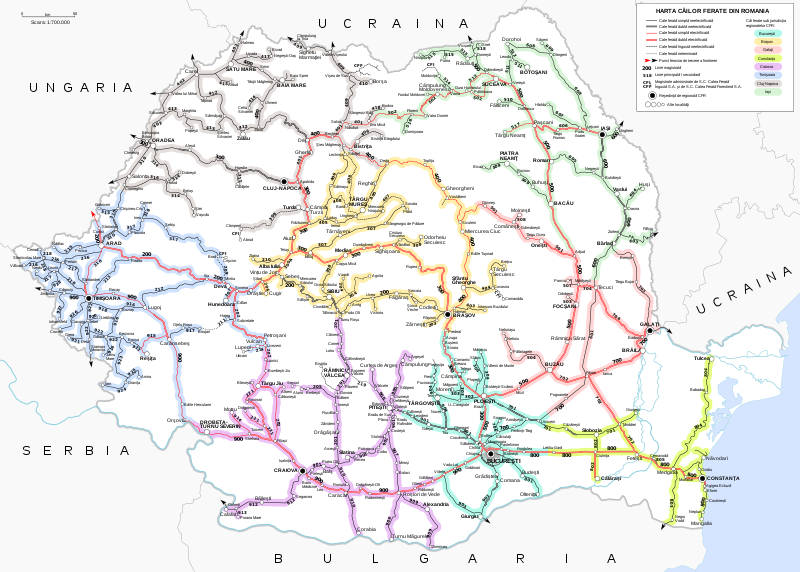
\includegraphics[width=0.8\textwidth]{./figures/ch3_romania-feroviara.png}
    \caption{Map of Romania's railway network. Map by Aero Avalon, shared under CC-BY 4.0 \cite{WikipediaRomaniaFeroviara}.}
    \label{FigRomaniaFeroviara}
\end{figure}

The passenger subsidiary, CFR Călători, is the biggest railway operator that makes use of these lines. However, rolling stock is outdated and most train cars lack modern features like driver-controlled doors. A notable absence though is that of live travel information offered inside the train to the passengers. An example of such an information display is given in Figure \ref{FigMAVInterior}.

\begin{figure}[htbp]
    \centering
    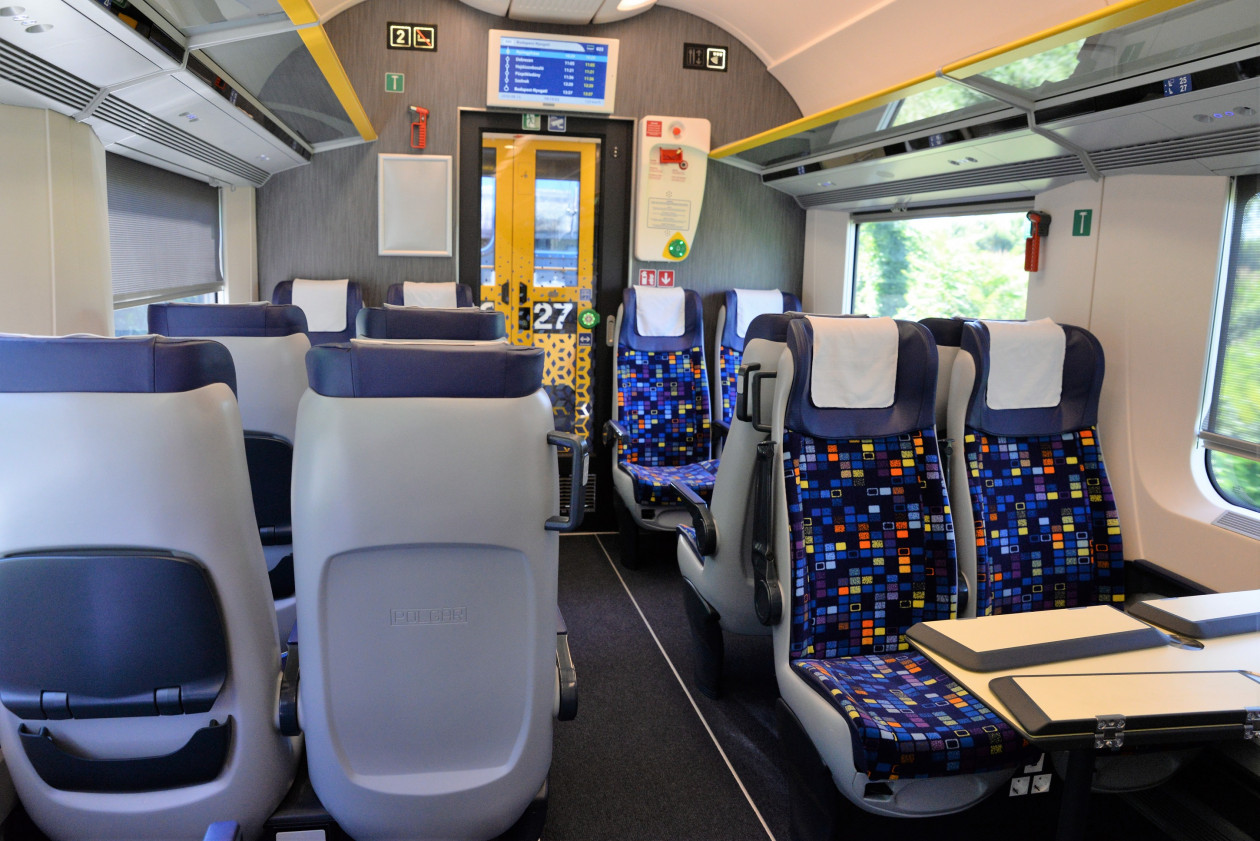
\includegraphics[width=0.8\textwidth]{./figures/ch1_mav-interior.png}
    \caption{Interior of a train owned by MÁV-Start, the Hungarian national passenger operator \cite{PestiHirlapMAVInterior}. The LCD display can be seen at the top, providing information about the next stations, times and delays. Stations and times can be pre-programmed into the train on departure, but delays require live integration with a central service.}
    \label{FigMAVInterior}
\end{figure}

Given that retrofitting all rolling stock with displays connected to the Internet is a challenging task, CFR Călători has attempted digitization in various other ways.

In 2016, the company launched IRIS, a web application that provided traffic information about the company's trains. It also offered information about delays \cite{StiriDeClujLansareCFRIris}. In 2018, IRIS got discontinued in favor of a newer platform, written in ASP.NET, which offers information about all railway operators in Romania.

In 2021, the company launched a mobile application with all the capabilities that the website has, making it more convenient than ever before to view traffic information \cite{MobilissimoCFRLansareMobil}.

These solutions, however, are insufficient in answering the question of "Where am I?" that a passenger might have. The most significant issue is that they all require Internet, the lack of which is an issue prevalent across Romanian trains \cite{CFRInternetIC}.

Moreover, CFR does not track the location of their trains using GPS transponders or any similar technology, but rather using personnel that are responsible with coordinating the trains passing through each station. This brings a number of issues:

\begin{itemize}
    \item \textbf{Data is not real-time.} A train passing through a station is only recorded when the station personnel manually records that train as passed, in the company's internal services.
    \item \textbf{Data might be missing.} Some personnel might not take the time to enter delay data for each passing train.
    \item \textbf{Some stations are not tracked.} Some train stations are big enough to be serviced by regional trains, but not big enough to warrant any personnel responsible with train movement.
    \item \textbf{Data might be false.} Station personnel can enter any delay data they want, having the possibility of hiding delays.
\end{itemize}

\section{Application requirements}
\label{sec:Requirements}

Given the set of real-world issues mentioned above, we can create a set of requirements for an application that tries to plug the information gap and provide a seamless travel experience for the passenger.

The basic idea of this thesis is to merge the mobile app experience and the website experience offered by CFR into a single solution, that will then be extended to offer live traffic information using phone capabilities such as the camera and location.

\begin{enumerate}
    \item Train trip information
          \begin{itemize}
              \item The app should allow the user to create a new trip. The user will be able to view live information about this trip.
              \item The app should be able to show details about the user's current position in their trip, using information obtained from user (train ticket), train database (itinerary of train) and phone sensors (GPS location).
              \item The live information should include: next stop, last stop, next stop arrival time (timetabled), train delay, next station of pass-through (if applicable).
              \item The live information may also include the destination arrival time (time\-tabled) + train delay.
              \item Information about the train ticket can be obtained using multiple methods: scanning the QR code of the ticket (state operator only), or manually inputting ticket data (train number, destination station).
              \item Access to non-live data should be provided via links to the Mersul Trenu\-rilor website (train itinerary, station stops).
              \item National train itinerary information will be saved to the user's device on application install. The information can be updated from the server. Attempts to automatically update this data will be done weekly.
          \end{itemize}
    \item User profile and authentication
          \begin{itemize}
              \item The app should be able to be used anonymously, without login. If so, persistent data must be saved locally to the device.
              \item The app must provide social login (login with Google, login with Apple) as the primary means of logging in.
              \item When creating a new account (logging in for the first time), if there is local data on the device, the app must offer the user the possibility of migrating it to the account. If logging into an existing account, local data must be deleted.
              \item The app must be able to show to the user a history of their trips.
              \item Logging in on another device will log out the already-logged-in device.
          \end{itemize}
    \item Connectivity
          \begin{itemize}
              \item The app must work without Internet, except for functionalities that directly require it.
              \item Account login will not work without Internet.
          \end{itemize}
          \item{Internationalization}
          \begin{itemize}
              \item The app must provide multi-language support (Romanian and English).
          \end{itemize}
\end{enumerate}

\section{Guiding principles}

To maximize user adoption and ease of use, the application should be centered about these core principles:

\begin{itemize}
    \item \textbf{Offline:} it will work at maximum capability while offline.
    \item \textbf{Easy to get into:} users should be able to get live tracking as soon as they click a link, and should not have to install apps.
    \item \textbf{Live information:} the screen will update as soon as the app gets new traffic or position information.
    \item \textbf{Information at a glance:} all information needed to answer the questions of "Where am I?", "How long until next stop?", "How long until my stop?" is always displayed on-screen.
    \item \textbf{Minimal configuration:} integrate with existing CFR services and ticketing systems as seamlessly as possible.
    \item \textbf{Avoid "yet another account and password":} allow the user to save their preferences locally, or use social login to sync them. Do not ask the user to remember another password!
\end{itemize}

\section{Use case diagram}

We can also design a use case diagram showing the main functionalities of the application and how we intend them to interoperate and operate with the various actors, in Figure \ref{FigUseCase}.

\begin{figure}[htbp]
    \centering
    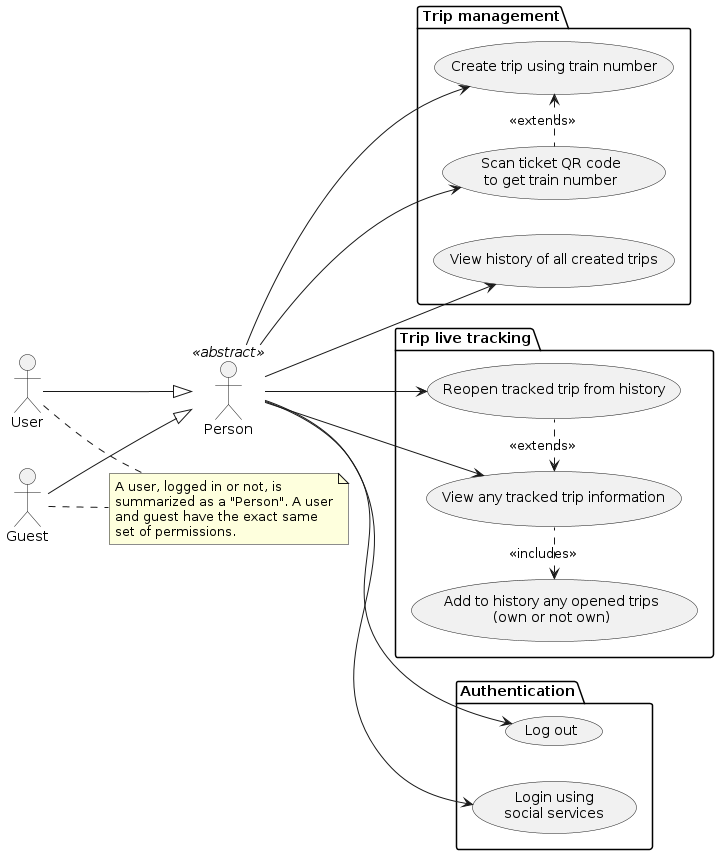
\includegraphics[width=0.9\textwidth]{./figures/ch3_use-case.png}
    \caption{Use case diagram for our CFR Companion application.}
    \label{FigUseCase}
\end{figure}

As you can see, even though we employ user accounts, there is little operational difference between users that are logged in, and those who are not. The permission set is the same, what is different is where the user data (trip history) is saved.

\iffalse
    \section{MOMENTARILY DISCARDED: User stories}

    Given the set of core principles outlined in the previous section, a list of user stories can be compiled. Features that are \textbf{not} necessary for a Minimum Viable Product (MVP) are marked as such and are de-prioritized.

    A minimum viable product, in our case, comprises the set of features needed to fullfil our core principles.

    I used the shorthand "AaU" to mean "As a User".

    \begin{tabularx}
        {\linewidth}{
            | >{\hsize=.15\hsize}X
            | >{\hsize=.65\hsize}X
            | >{\hsize=.2\hsize}X |
        }
        \hline
        Category / Story \# & User story                                                                                                           & Scope        \\
        \hline\hline
        \multicolumn{3}{|X|}{1. Live Location}                                                                                                                    \\
        \hline 1.1.         & AaU, I want to see live where I am, what's the next station, and when I get there                                    & MVP          \\
        \hline 1.2.         & AaU, I want to manually input my train number so that the app knows                                                  & MVP          \\
        \hline 1.3.         & AaU, I want to be able to make a picture of my ticket so that the app can figure out my train number                 & Nice to have \\
        \hline 1.4.         & AaU, I want to be able to scan the ticket's QR code so that the app can figure out my train number                   & Nice to have \\
        \hline 1.5.         & AaU, I want to send a screenshot of an online ticket (or the CFR PDF) so that the app can figure out my train number & Nice to have \\
        \hline 1.6.         & AaU, I want to see, live, what delay my train has                                                                    & MVP          \\
        \hline 1.7.         & AaU, I want to see, live, what the next and last stations are                                                        & MVP          \\
        \hline 1.8.         & AaU, I want to see intermediary stations where the train doesn't stop                                                & Nice to have \\
        \hline 1.9.         & AaU, I want to see, on a map, where I am                                                                             & Nice to have \\
        \hline 1.10.        & AaU, I want to see what station I get off at, and see when I get there                                               & Nice to have \\
        \hline
        \hline
        \multicolumn{3}{|X|}{2. Schedules Information}                                                                                                            \\
        \hline 2.1.         & AaU, I want to see, for a station, what trains arrive there, and at what times                                       & MVP          \\
        \hline 2.2.         & AaU, I want to see, for my train, all stations it has                                                                & MVP          \\
        \hline 2.3.         & AaU, I want to see, for my train, all intermediary stations that it does NOT stop at                                 & Nice to have \\
        \hline
        \hline
        \multicolumn{3}{|X|}{3. User profile and Authentication}                                                                                                  \\
        \hline 3.1.         & AaU, I want to be able to use the app anonymously                                                                    & MVP          \\
        \hline 3.2.         & AaU, if I create an account, I want to be able to merge my data into the account                                     & Nice to have \\
        \hline 3.3.         & AaU, I want to be able to register/login using my Apple account                                                      & MVP          \\
        \hline 3.4.         & AaU, I want to be able to register/login using my Google account                                                     & MVP          \\
        \hline 3.5.         & AaU, I want to be able to optionally set up 2FA using an Authenticator app                                           & Nice to have \\
        \hline 3.6.         & AaU, if I have 2FA on, I want to be able to login using a recovery code                                              & Nice to have \\
        \hline 3.7.         & AaU, I want to add a train trip to my history, manually                                                              & MVP          \\
        \hline 3.8.         & AaU, I want to have any ticket I scan added automatically to my history                                              & Nice to have \\
        \hline 3.9.         & AaU, I want to see the history of my train trips                                                                     & MVP          \\
        \hline 3.10.        & AaU, I want to see a digest of my history: most visited station, most traveled-on route, etc                         & MVP          \\
        \hline
        \hline
        \multicolumn{3}{|X|}{4. Internationalisation}                                                                                                             \\
        \hline 4.1.         & AaU, I want to be able to select a language I prefer to see the app in (EN / RO)                                     & MVP          \\
        \hline
        \hline
        \multicolumn{3}{|X|}{5. Appearance}                                                                                                                       \\
        \hline 5.1.         & AaU, I want to be able to select a dark or light theme                                                               & Nice to have \\
        \hline
    \end{tabularx}
\fi